AFGMiner generates and tests candidate patterns of increasing number of edges, then extends those patterns considered heavyweight. It generates candidate patterns of $k$ edges, starting with $k = 0$ (patterns composed of a single node and no edges), and searches for occurrences of such patterns in the dataset by using a sub-graph isomorphism detection algorithm. Each ocurrence found has its node weight and edge weight support values computed, and, when no more occurrences of a pattern are present in the dataset, the support value for the pattern itself is computed by aggregating the support values of its occurrences. If the support value for the pattern is higher than an user-defined threshold, the pattern is heavyweight. It is then output to the user and later extended into candidate patterns with an additional edge, a process called \emph{edge-by-edge pattern extension}. If the pattern is not heavyweight, it is discarded. 

Edge-by-edge pattern extension works by adding to a pattern either: (i) an edge that connects two of its nodes; (ii) or an edge that connects one of its nodes to a new node called the \emph{extension node}. A pattern that generates other patterns by extension is called a \emph{parent pattern}, while the generated patterns are \emph{child patterns}.

\subsection{Canonical Labeling}
Two different patterns, when extended, may generate child patterns that are isomorphic. It is inefficient to mine for redundant patterns, so redundancy should be detected. The well-known concept of \emph{canonical labeling} of patterns is used to detect redundancy~\cite{gSpan}. The idea is to map each sub-graph pattern to an identifier string called \emph{DFS Code}. The string representation, or DFS Code of an AFG of $n$ edges is $(e_0) (e_1)...(e_n)$, where each edge $e_i=(v_i, v_j)$ is represented by a string: $( [l(v_i):$ $(a_{i_0})$ $(a_{i_1})...(a_{i_m})]$ $[l(v_j): (a_{j_0}) (a_{j_1})...(a_{j_p})] )$, where $m$ and $p$ are the number of attributes present in the edge's \emph{from-node} and \emph{to-node}, respectively. DFS Codes can be lexically ordered in such a way that, if two sub-graphs are isomorphic to each other, they provably have the same minimum DFS Code. The rules that define how to sort DFS Codes depend on the types of graphs being mined. 

In order for a newly-generated sub-graph pattern to be considered redundant, and thus discarded, its DFS Code should be already present in $H$, a hash-set whose elements are the distinct DFS Codes of all patterns that have been processed. However, this approach may consume large amounts of memory because the number of candidate patterns generated may be very high. Instead, the approach adopted in the prototype implementation of AFGMiner is to record the DFS Codes only for patterns considered heavyweight. 

When producing the DFS Code of a sub-graph pattern, it is a requirement to label the edges and nodes of the pattern. Nodes are labelled as follows. The attribute set of the node is used as its preliminary label, by forming a bit vector in which each attribute is represented by a bit presence or absence of the attribute. Edge labels are simply the labels of the edges's \emph{from-node} and \emph{to-node} in that order. The edge labels are sorted by considering that, given any two edge labels, the one with the lower \emph{from-node} label comes first, and in case those are the same, the one with the lower \emph{to-node} label comes first. The minimum DFS spanning tree of the sub-graph pattern is then computed using the sorting order of the edge labels \emph{in lieu} of edge weights. Finally, the order in which pattern nodes are visited during a pre-order traversal of this minimum spanning tree determines their final and unique-per-pattern label, which is used to sort the edges. The resulting sorted edge labels of two patterns is the same if the patterns are isomorphic.

\subsection{Support Value Policy}
The process of generating and testing candidate patterns in AFGMiner may be understood as the exploration of the space of patterns that exist in the dataset of AFGs being mined. The algorithm searches for all the heavyweight patterns present in this space, which can be envisioned as a forest of trees with the root node of each tree being a 0-edge pattern, child nodes of the root node being the 1-edge patterns extended from the 0-edge patterns, etc. Pruning this search space as much as possible is desirable in order to decrease the run-time of the algorithm. AFGMiner adopts an \emph{anti-monotonic} support value policy to enable the pruning of the search space. Under this policy, the support value of a pattern is always lower than or equal to the support value of any of its ancestor patterns. Therefore, if a pattern is not heavyweight, none of its descendants can be heavyweight. Thus all patterns that do not meet a minimum support criteria can be discarded. The anti-monotonic support value policy allows the algorithm to prune  nodes in the search space that it identifies as non-heavyweight patterns. 

The support value policy works as follows. For each occurrence $g$ of a pattern $p$, two values are calculated: $S_n(g)$, the weight of the attribute with minimum weight amongst all attributes associated with nodes of $g$; and $S_e(g)$, the minimum edge weight amongst all edges of $g$. The $S_n(g)$ of all occurrences of $p$ found in $DS$ are then added up, resulting in $S_n(p)$, the node weight support of $p$. The $S_e(g)$ of all occurrences of $p$ found in $DS$ are also added up, resulting in $S_e(p)$, the edge weight support of $p$. The support value for $p$ is $S_m(p)$, the maximum between $S_n(p)$ and $S_e(p)$. $S_m(p)$ is compared against the support threshold to decide whether $p$ is a heavyweight pattern. 

The principle behind separately computing the support values of node attributes and edges of a pattern and then choosing the maximum between the two values is that a pattern is relevant if either, or both, the attributes or edges of its occurrences have significant weight in comparison to the sum of all node weights and to the sum of all edge weights in the dataset. The support-value policy selected for AFGMiner is conservative because only the minimum edge weight and the minimum node attribute weight of each occurrence are used in the computation. Less conservative support-value policies could be adopted as long as they are anti-monotonic.  

\subsection{Matching Patterns to Occurrences}
When a candidate pattern is generated, its DFS Code is computed and the algorithm checks if the DFS Code already exists in $H$. If the DFS Code is not present, the candidate pattern is not redundant and the process of mining for it in the dataset begins. The mining process finds sub-graphs $g$ in AFGs of $DS$ that match the candidate pattern $p$. AFGMiner may use any sub-graph isomorphism detection algorithm to match patterns and sub-graphs, as long as the algorithm is adapted to take node attributes into consideration when detecting isomorphism. The prototype implementation of AFGMiner adapts VF2~\cite{Cordella}, an algorithm that is faster than alternatives for graphs that are relatively regular, have a large number of nodes and whose nodes have small valency~\cite{Foggia}. For the case study described in this paper, AFGs meet this criteria. 

VF2 produces a mapping $M$ between nodes in $p$ and nodes in $G$, where $G$ contains at least as many nodes as $p$. $M$ is expressed as a set of pairs $\{n, m\}$, where $n \in p$ and $m \in G$ are nodes. The mapping is said to be an isomorphism if $M$ is a bijective function that preserves the branch structure of both $p$ and $G$. This mapping is represented as a state $s$ in a State Space Representation (SSR). This state, which we call a \emph{miner state}, goes from empty (no mapping between nodes in $p$ and nodes in $G$) to a goal state (all nodes in $p$ mapped to respective nodes in $G$) during the process of finding $M$. A state transition between any miner state $s_1$ and its successor $s_2$ represents the addition of a new pair $\{n, m\}$ to the collections of known pairs that compose $M$. The addition of new pairs only occurs if $n$ and $m$ form a feasible pair. The rules for a pair of nodes to be considered feasible, in the case of AFGs, are as follows: (i) attributes of $m$ should be a proper superset of attributes in $n$; (ii) topological structure around $n$ and $m$ should be the same.

\subsection{Generation of Candidate Patterns}
The input to AFGMiner is a list $A_0$ of attributes that occur in the dataset. Each one of the possible attributes is used to create a set of 0-edge candidate patterns with a single attribute in their nodes, as shown in Figure~\ref{fig:example_0-edge}. The support value threshold in this example is $T = 1/23$. Each one of the candidate patterns $p$ is mined for in the dataset $DS$, and, if $p$ is heavyweight, its only attribute is added to $A_1$. $A_1$ is the list of distinct attributes that belong to 0-edge heavyweight patterns and that are used in the generation of 1-edge candidate patterns. 

After all 0-edge heavyweight patterns of a single attribute are found, the attributes in $A_1$ are combined in pairs and AFGMiner searches for the generated 0-edge candidate patterns that have two attributes each (Figure~\ref{fig:example_0-edge_2-attribute}). The attributes that compose the 0-edge candidate patterns of two attributes found to be heavyweight are then combined into sets of three attributes, which form the 0-edge candidate patterns of three attributes each. This continues until no more 0-edge heavyweight patterns with a certain number of attributes can be found. 

The process of mining for candidate patterns with an increasing number of attributes in their single node (in the case of 0-edge patterns) or in their extension node (in the case of $k$-edge patterns with $k > 0$) is called \emph{attribute-set growth}. Attribute-set growth is useful because an attribute set is only used to generate a pattern if all of its sub-sets generated heavyweight patterns. 

Each one of the 0-edge heavyweight patterns spans multiple child candidates, one for every attribute in $A_1$, in which the extension node contains a single attribute from $A_1$. Thus, all the pairs of nodes connected by an edge in Figure~\ref{fig:example_1-edge} are child candidates for the example. AFGMiner searches for matches for each candidate child pattern in the dataset as soon as the pattern is generated. If a candidate pattern is found to be heavyweight, all its attributes are added to $A_2$. Attributes in $A_2$ are then used to generate 1-edge candidate patterns that have two attributes in their extension node.  In Figure~\ref{fig:example_1-edge_2-attribute} a candidate is generated for each pair of nodes connected by an edge. For clarity, only candidates generated by the pattern $a$ $\rightarrow$ $a$ are shown. The attribute-set growth process then proceeds until no more 1-edge candidate patterns of certain number of attributes in their extension node can be found. In Figure~\ref{fig:example_2-edge}, 2-edge patterns are shown. 

A set of patterns that have the same number of edges is called a \emph{generation}. AFGMiner produces and mines for candidate patterns generation by generation as described above. Patterns of a certain generation are only created and mined after all the heavyweight patterns of the previous generation have been found. This is important because it allows the algorithm to use only the $A_k$ set of distinct attributes present in the $(k - 1)$-th generation to compose the patterns of the $k$-th generation, thus restricting the number of candidate patterns produced.

\begin{figure}[h!]
\centering
    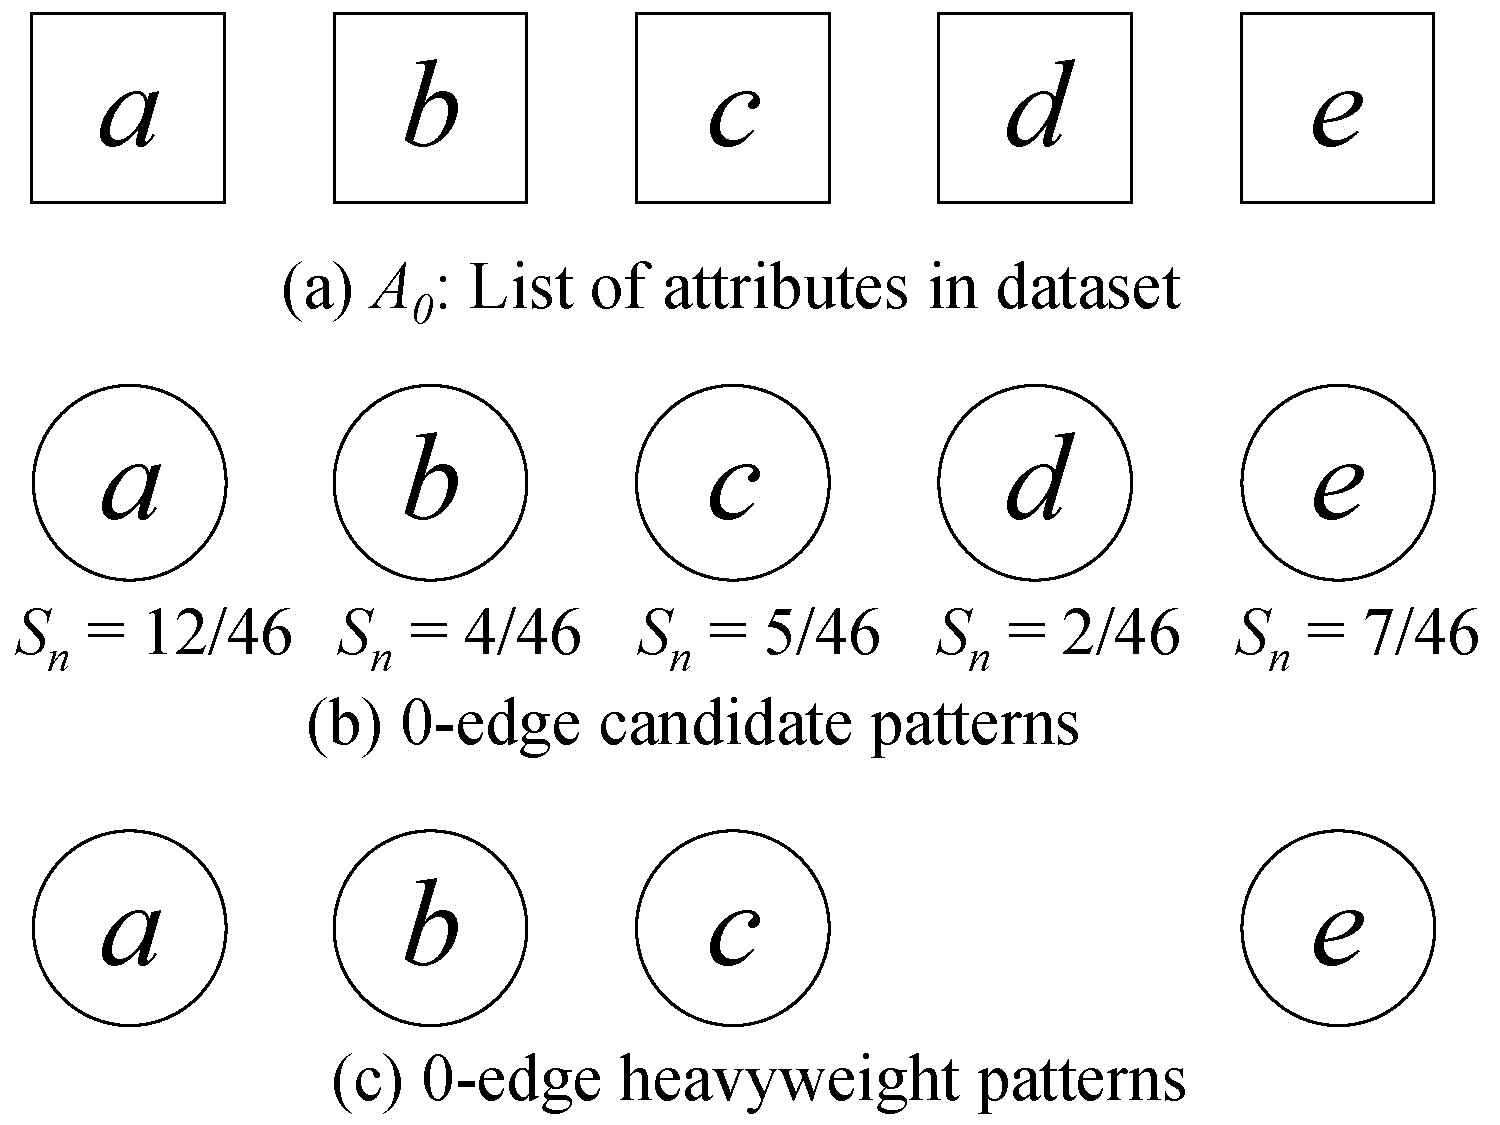
\includegraphics[scale=0.15]{figures/example_0-edge.pdf}
    \caption{0-edge candidate patterns.}
    \label{fig:example_0-edge}  
\end{figure}

\begin{figure}[h!]
\centering
    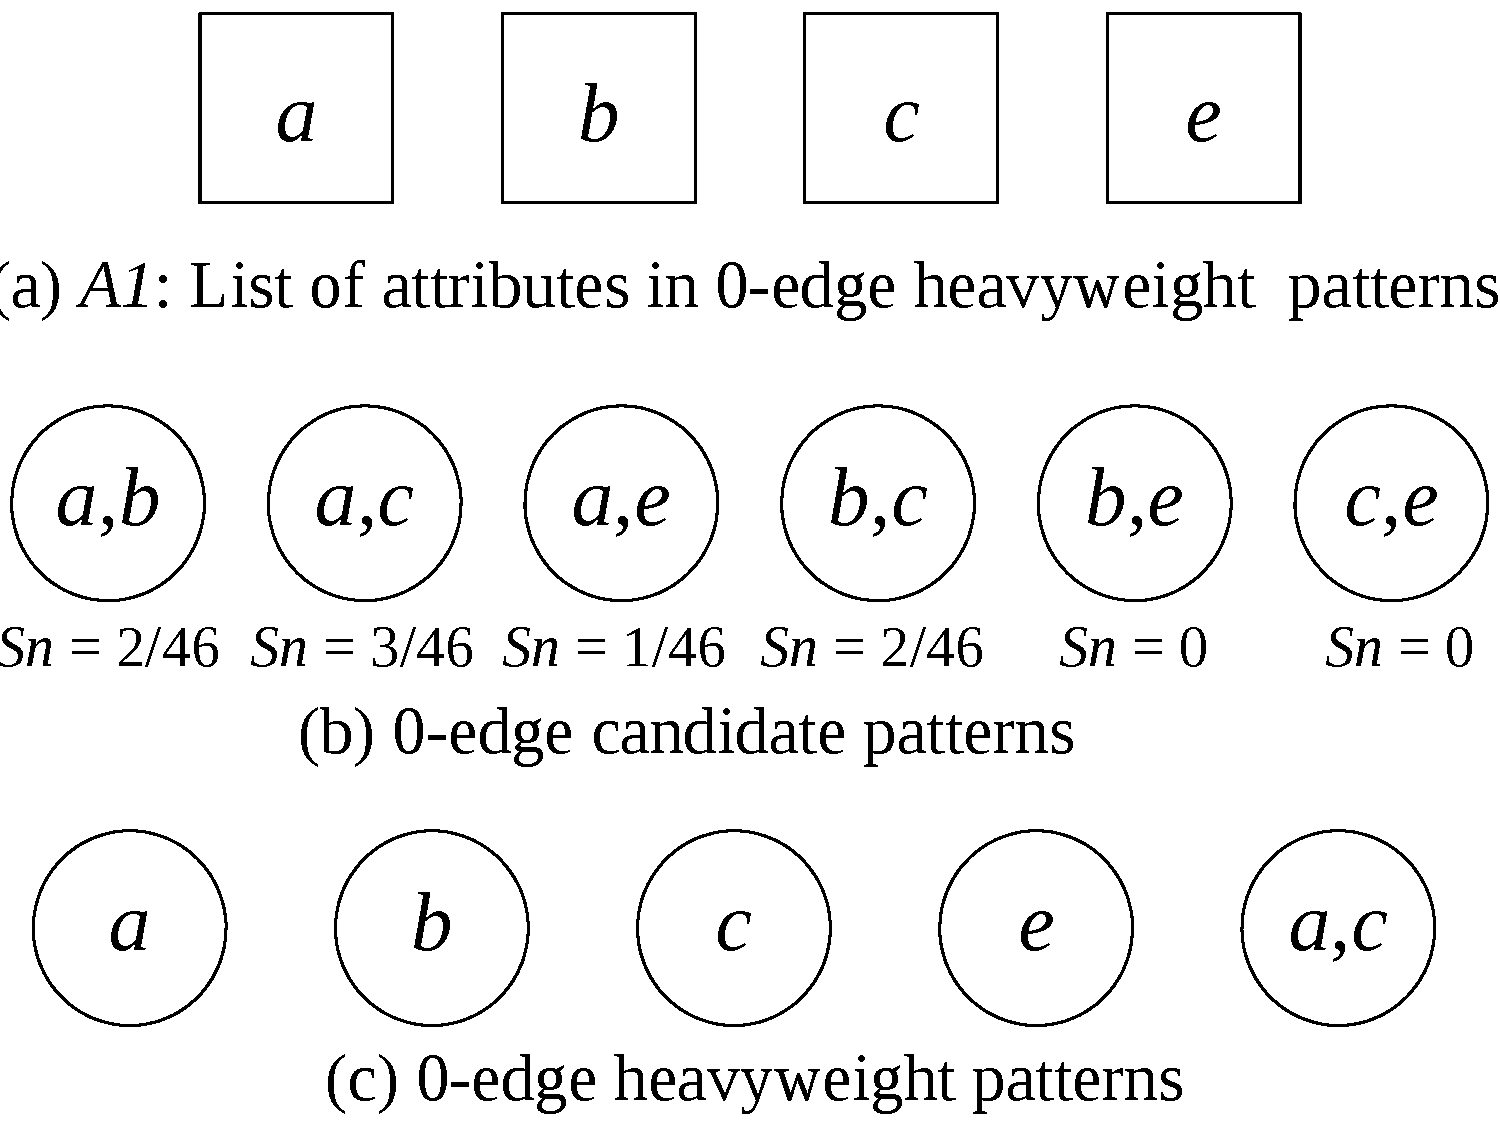
\includegraphics[scale=0.15]{figures/example_0-edge_2-attribute.pdf}
    \caption{Attribute-set growth for 0-edge candidate patterns.}
    \label{fig:example_0-edge_2-attribute}  
\end{figure}

\begin{figure}[h!]
\centering
    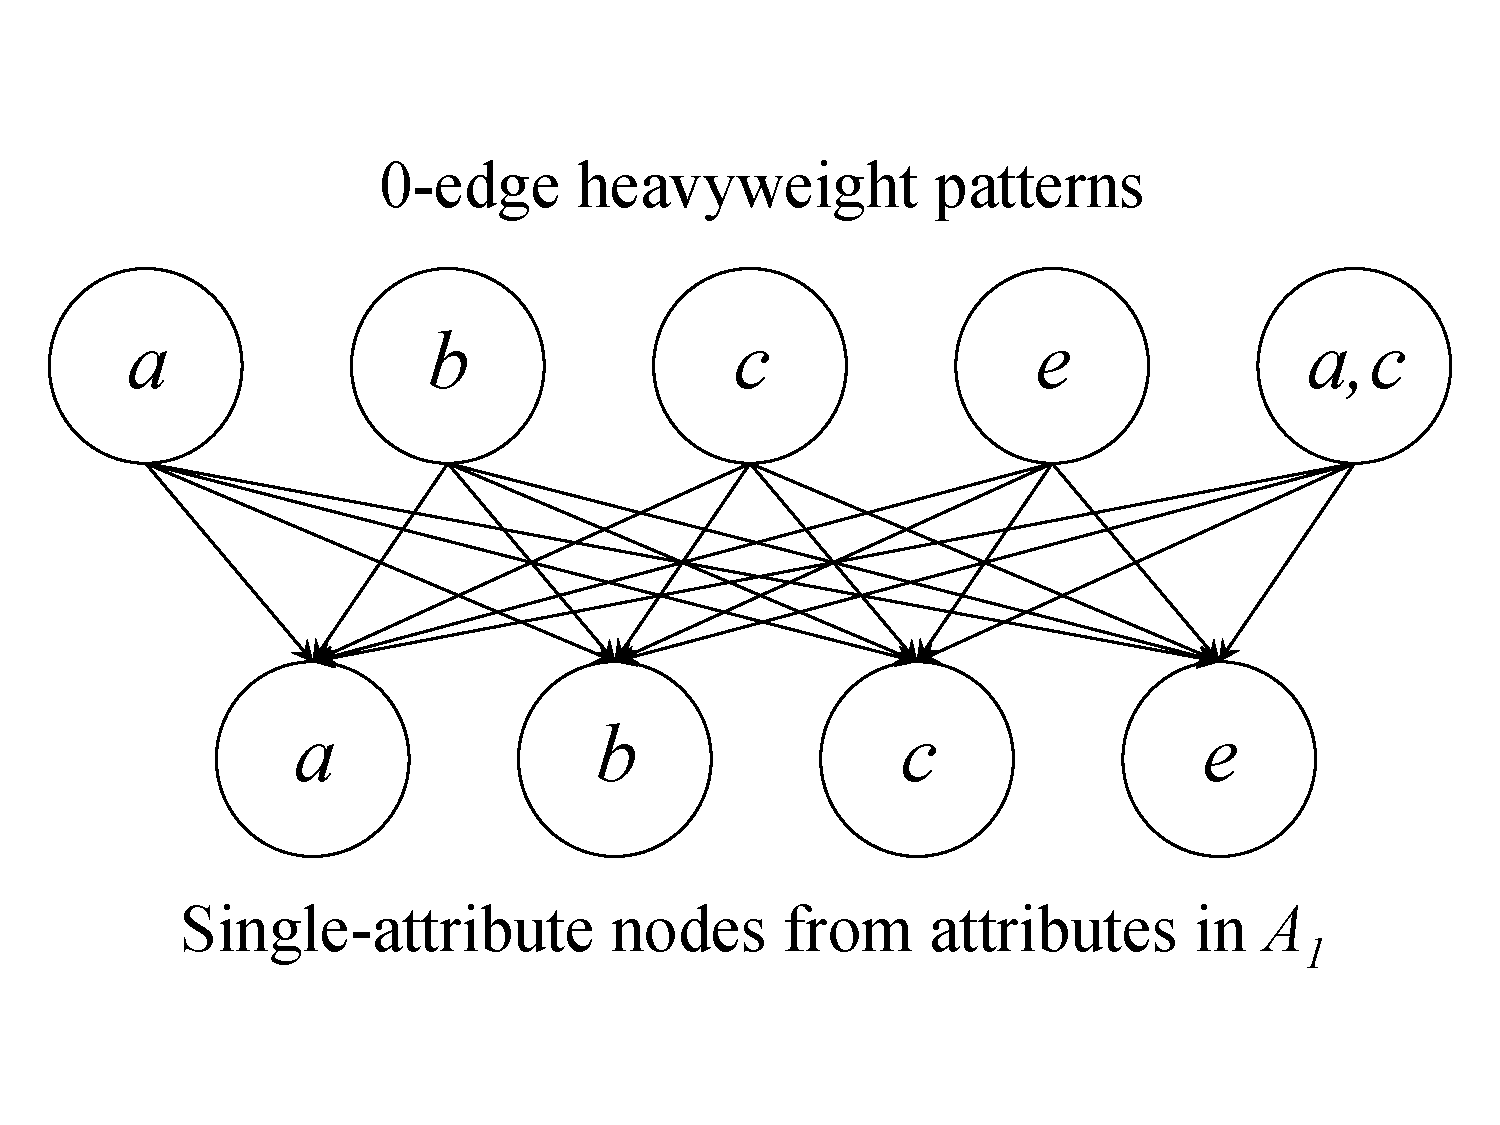
\includegraphics[scale=0.15]{figures/example_1-edge.pdf}
    \caption{1-edge candidate patterns.}
    \label{fig:example_1-edge}  
\end{figure}

\begin{figure}[h!]
\centering
    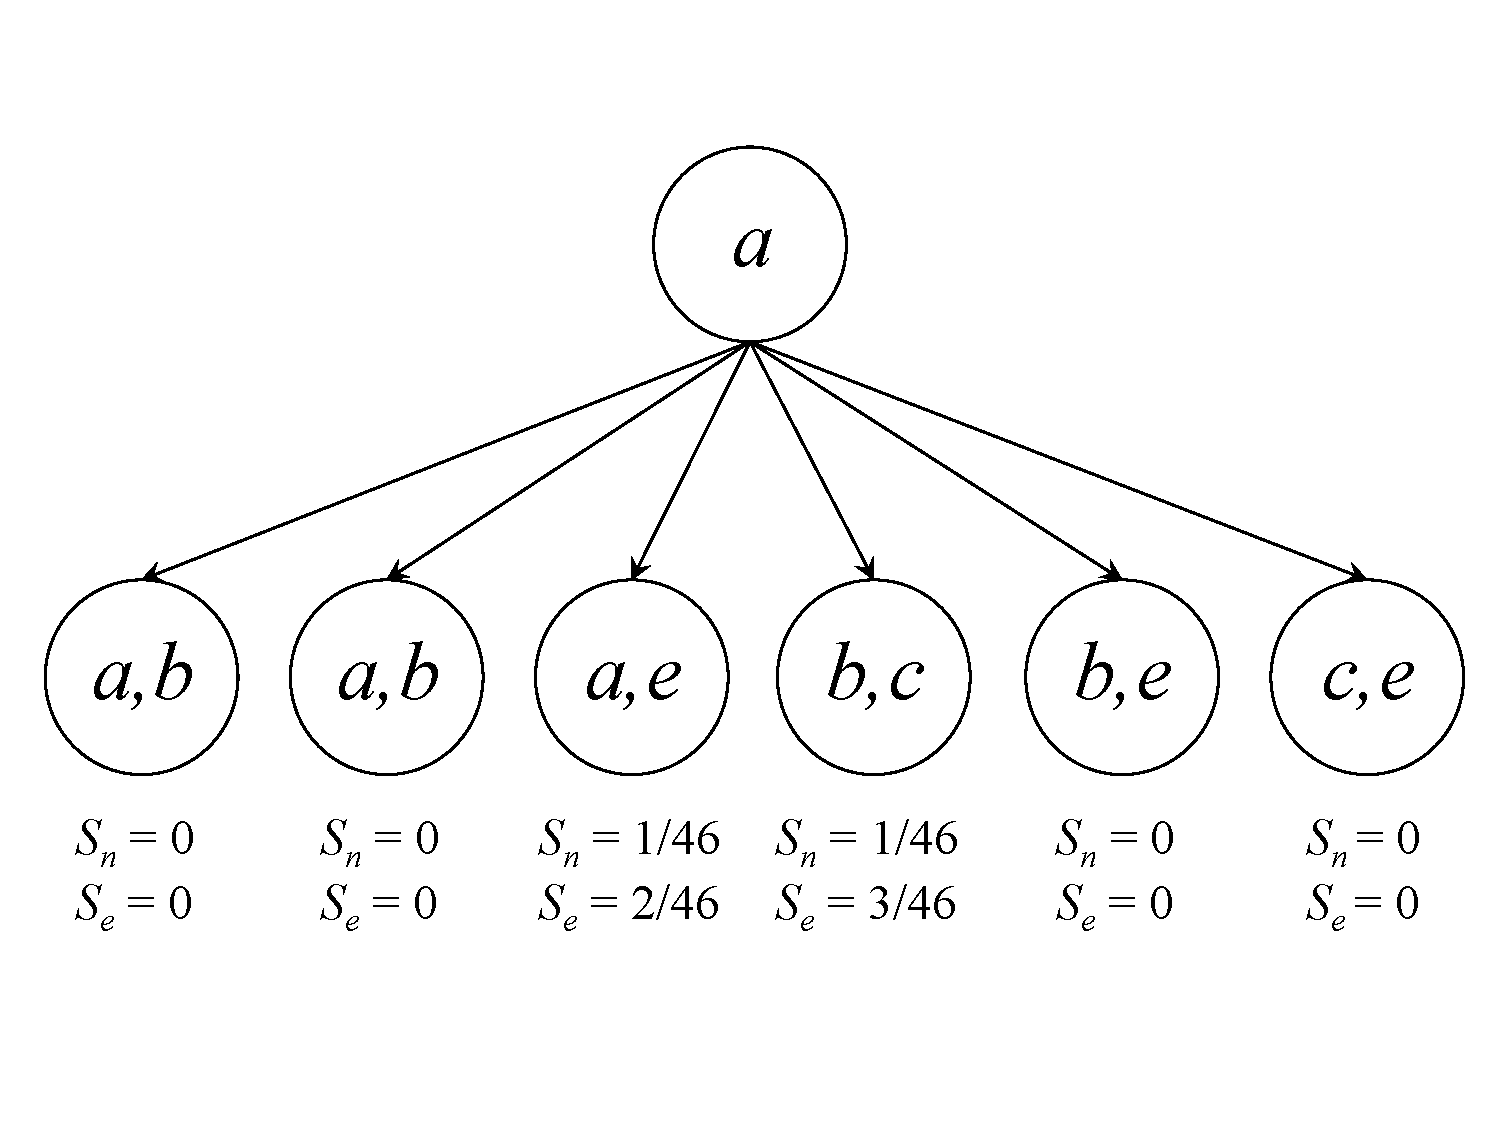
\includegraphics[scale=0.15]{figures/example_1-edge_2-attribute.pdf}
    \caption{Attribute-set growth for 1-edge candidate pattern node $a$ $\rightarrow$ $a$. }
    \label{fig:example_1-edge_2-attribute}  
\end{figure}

\begin{figure}[h!]
\centering
    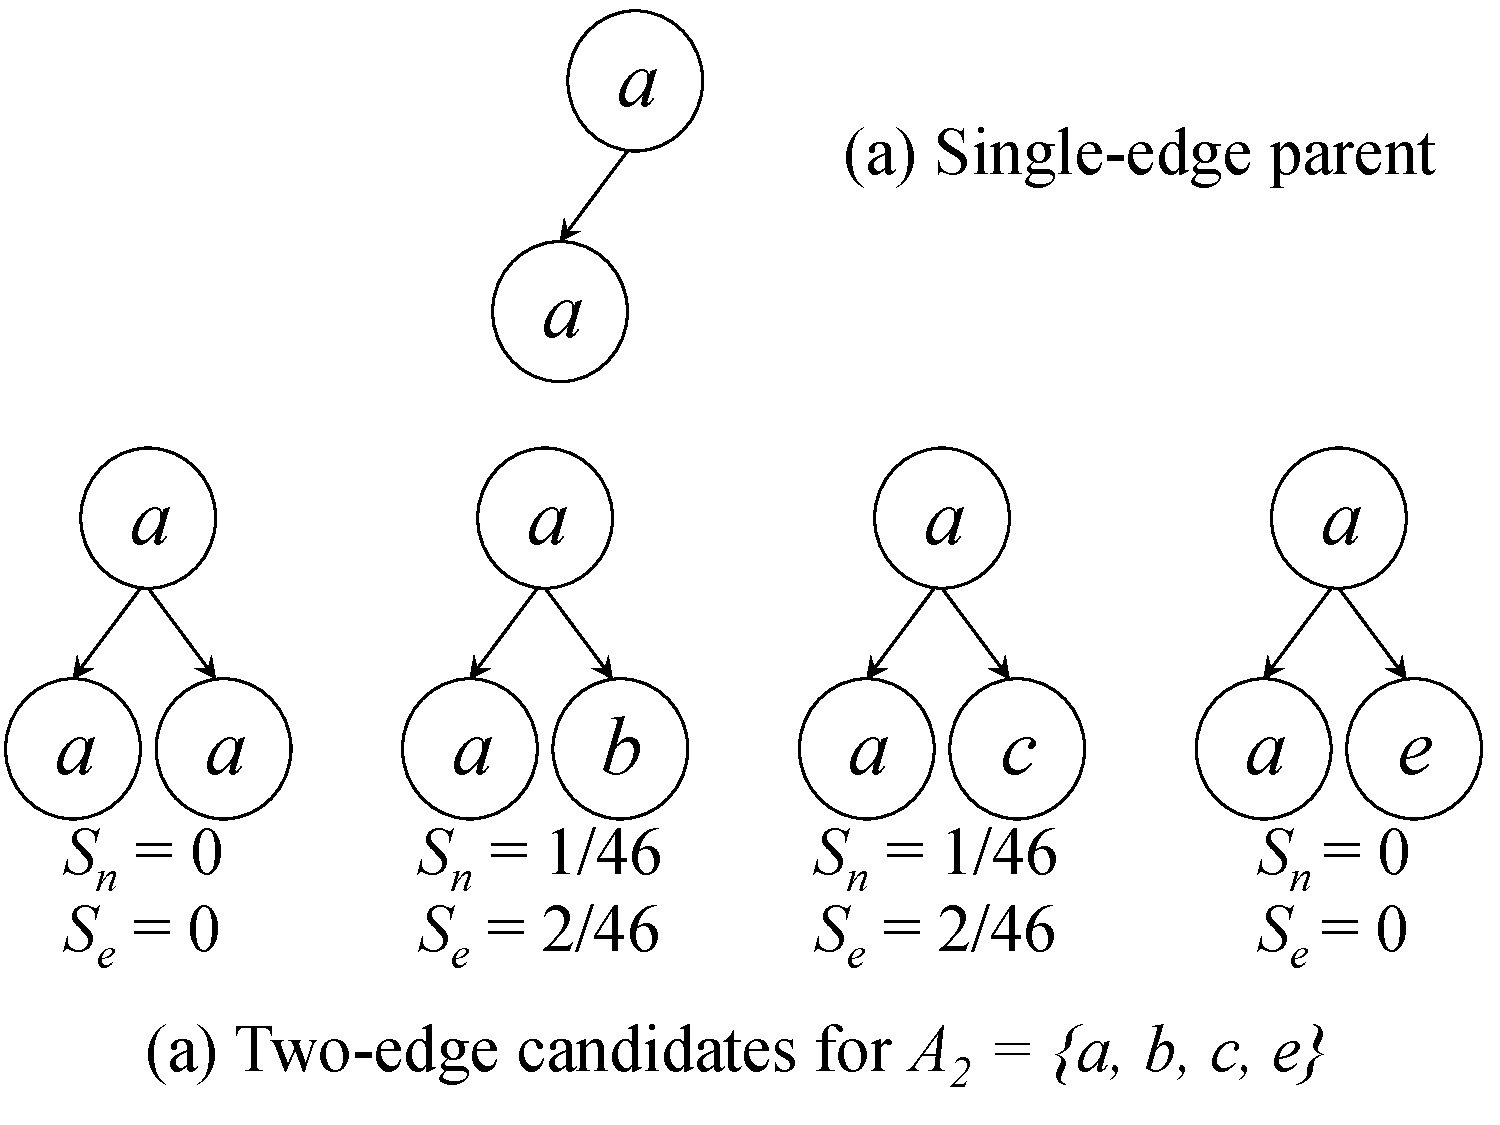
\includegraphics[scale=0.15]{figures/example_2-edge.pdf}
    \caption{2-edge candidate patterns.}
    \label{fig:example_2-edge}  
\end{figure}

